\mychapter{0}{KATA PENGANTAR}
%   \begin{figure}[h]
%     \centering
%     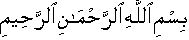
\includegraphics[width=0.5\linewidth]{images/bab0/gambarBismillah}
%   \end{figure}
	  Puji Syukur kepada Tuhan yang Maha Esa, atas berkatNya penulis dapat menyelesaikan buku berjudul \textbf{\judul}. 
	  \newline
	  \indent Selain itu, pada kesempatan ini penulis menghaturkan banyak terima kasih kepada pihak-pihak yang tanpa mereka, penulis tidak akan dapat menyelesaikan buku ini dengan baik :
  \begin{enumerate}
  	\item \textbf{\textit{Daddy Jesus}} - atas segala berkat, limpahan karunia, kesempatan dan rancangan jalanNya-lah penulis masih diberi nafas kehidupan, waktu, tenaga dan pikiran untuk menyelesaikan buku ini. \textit{Thank you, Big Daddy.}
    \item \textbf{Papa dan Mama} yang selalu menguatkan, menasehati, dan luar biasa sabar dalam mengingatkan penulis agar tidak lupa menjaga kesehatan dan tidak lupa ke gereja selama masa studi.
    \item \textbf{Yth Bapak Rully Soelaiman} yang mengajarkan penulis \textit{how to think scientifically} juga bimbingan, nasehat, saran dan memberikan penulis sisi pemikiran dan perspektif lain terhadap setiap masalah.
    \item \textbf{Yth Bapak Rizky Januar Akbar} sebagai dosen pembimbing yang memberi bimbingan, saran teknis dan administratif, diskusi dan pemecahan masalah dalam pembuatan dan penulisan buku tugas akhir.
    \item \textbf{Keluarga XL Future Leader Scholarship Camp Batch 5 \& KSE ITS} yang telah menyadarkan, memberikan semangat dan inspirasi untuk terus melanjutkan tugas akhir di saat penulis kehilangan semangat.
    \item \textbf{Keluarga Admin Lab. Pemrograman (2014 - 2017)} , yang telah memberikan penulis banyak pengalaman, pengetahuan dan cerita-cerita untuk dikenang.
    \item  \textbf{Keluarga Pengpro \textit{Furions} dan HMTC Optimasi 2016 }, yang mengajarkan penulis tentang cara berorganisasi, cara berbicara di depan publik, dan banyak lagi. 
    \item Bang Christo yang sudah jadi inspirasi dan semangat kuliah penulis sejak tahun pertama masa studi penulis sampai saat ini.  
    \item \textbf{Keluarga Alumni Budi Mulia Siantar-Surabaya angkatan 2013 } , teman setia disaat suka maupun duka. 
    \item Serta semua pihak yang tidak tertulis - yang telah turut membantu penulis dalam menyelesaikan Tugas Akhir ini.
  \end{enumerate}
  
  \indent Penulis menyadari bahwa Tugas Akhir ini masih memiliki banyak kekurangan. Oleh karena itu, penulis berharap kritik dan saran dari pembaca sekalian untuk memperbaiki buku ini ke depannya.

  \hfill Surabaya, Juni 2017 \\ \\ 


  \hfill Ronauli Silva N. Sidabukke

\cleardoublepage % Mengisi penanda halaman genap yang kosong

